\documentclass[a4paper, 11pt]{article}
\usepackage{comment} 
\usepackage{fullpage}
\usepackage{amsmath} 
\usepackage{amssymb} 
\usepackage{mathtools}
\usepackage{fontspec}
\defaultfontfeatures{Ligatures=TeX}
\usepackage{xfrac}
\usepackage{icomma}
\usepackage[section,below]{placeins}
\usepackage[labelfont=bf,font=small,width=0.9\textwidth]{caption}
\usepackage{subcaption}
\usepackage{graphicx}
\usepackage{grffile}
\usepackage{float}
\floatplacement{figure}{htbp}
\floatplacement{table}{htbp}
\usepackage{booktabs}
\usepackage{hyperref}
\usepackage[ngerman]{babel}
\usepackage{pdfpages}

\begin{document}
\noindent
%\centerline{\small{\textsc{Technische Universität Dortmund}}} \\
\large{\textbf{12. Übungsblatt zur Vorlesung \hfill WS 2017/2018 \\
Statistische Methoden der Datenanalyse \hfill Prof. W. Rhode}} \\
Annika Burkowitz, Sebastian Bange, Alexander Harnisch \\
\noindent\makebox[\linewidth]{\rule{\textwidth}{0.4pt}}

\section*{Aufgabe 36}
Rechnung angehangen.
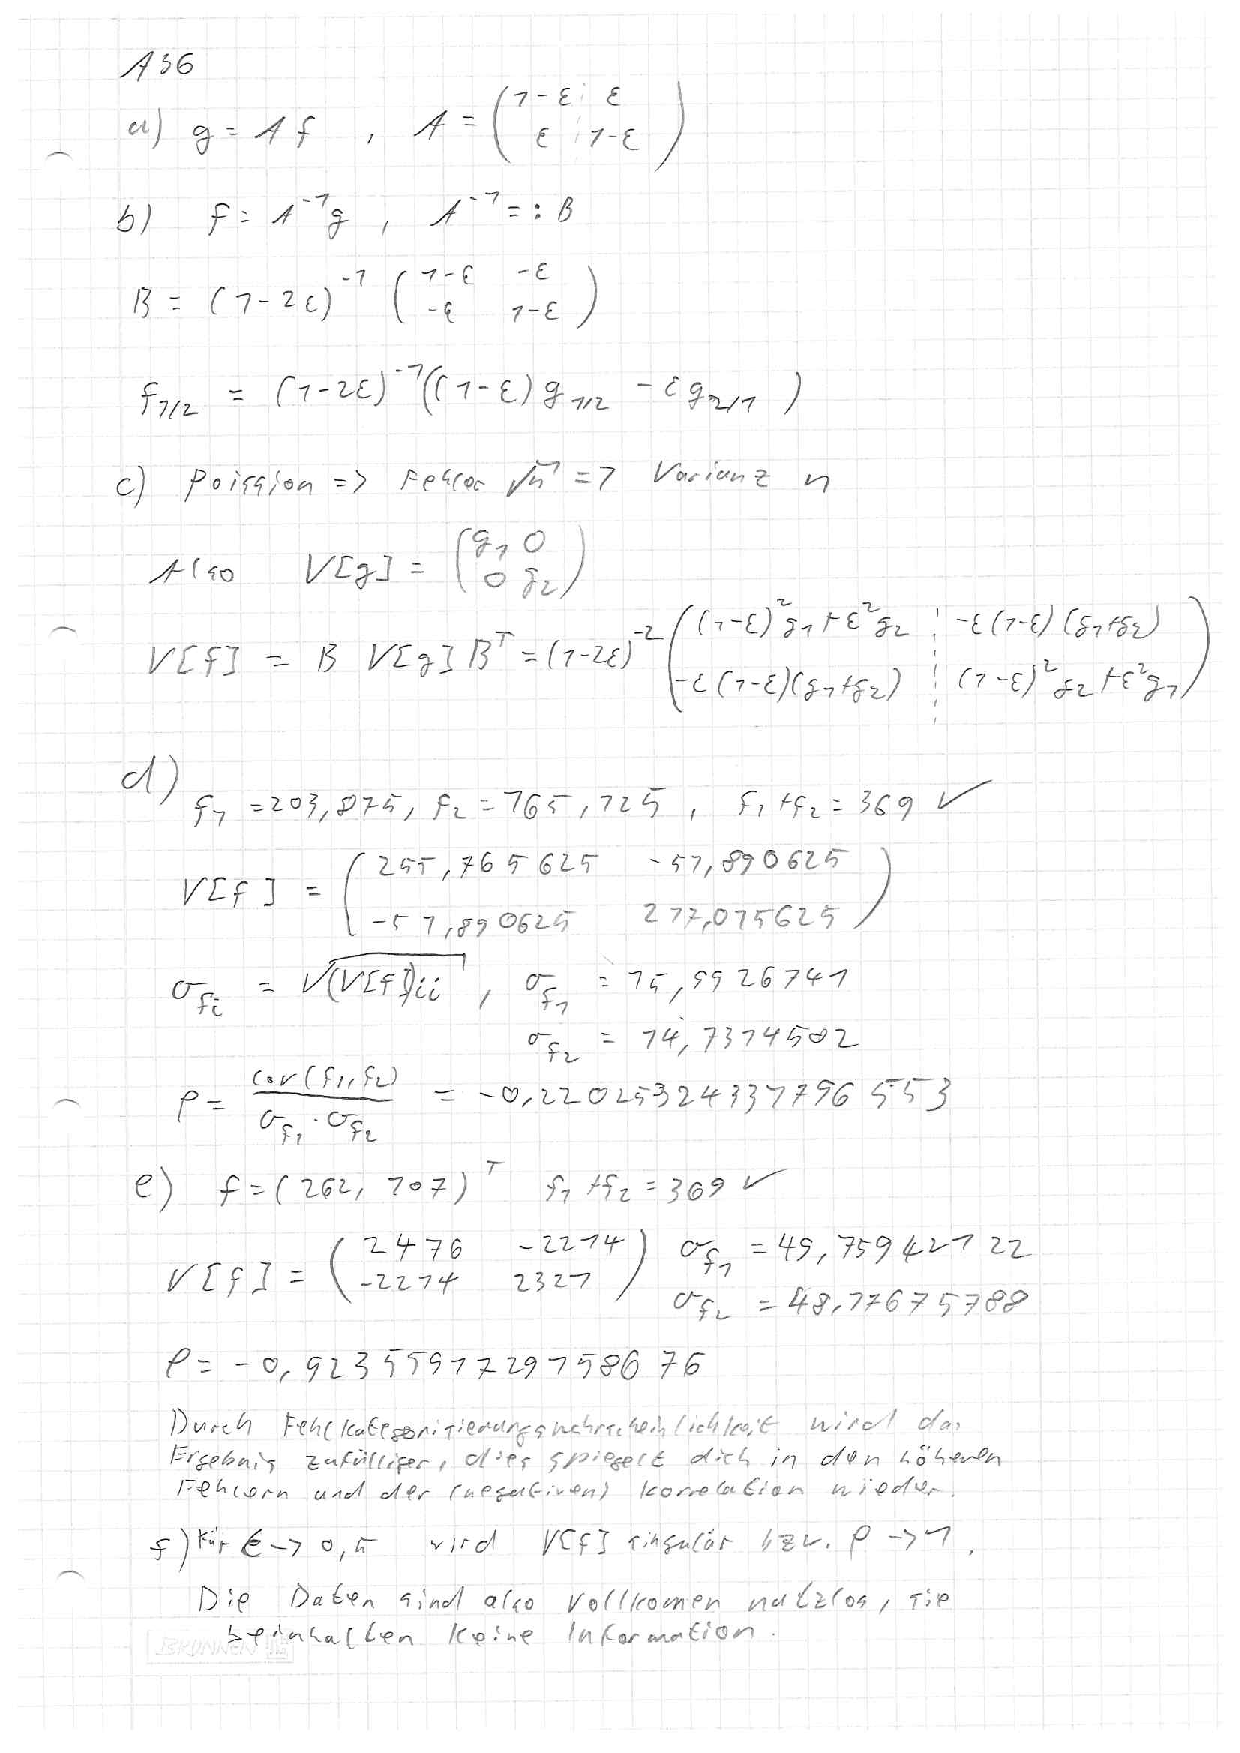
\includepdf[pages=1]{../Rechnungen.pdf}

\section*{Aufgabe 37}
Rechnung angehangen.
\subsection*{a)}
Es handelt sich um einen Messprozess, bei dem mit Wahrscheinlichkeit $\varepsilon$ ein Ereignis fälschlicherweise in den nächst höheren oder niedrigeren Bin kategorisiert wird, und daher mit Wahrscheinlichkeit $1 - 2\varepsilon$ in den korrekten (bzw. $1 - \varepsilon$ für die Randbins).
\subsection*{c)}
Die Eigenbasis hat, wie immer, den Vorteil, dass die Matrix hier diagonal ist daher lässt sie sich hier sehr leicht und stabil invertieren.
\subsection*{d)}
\begin{figure}
    \centering
    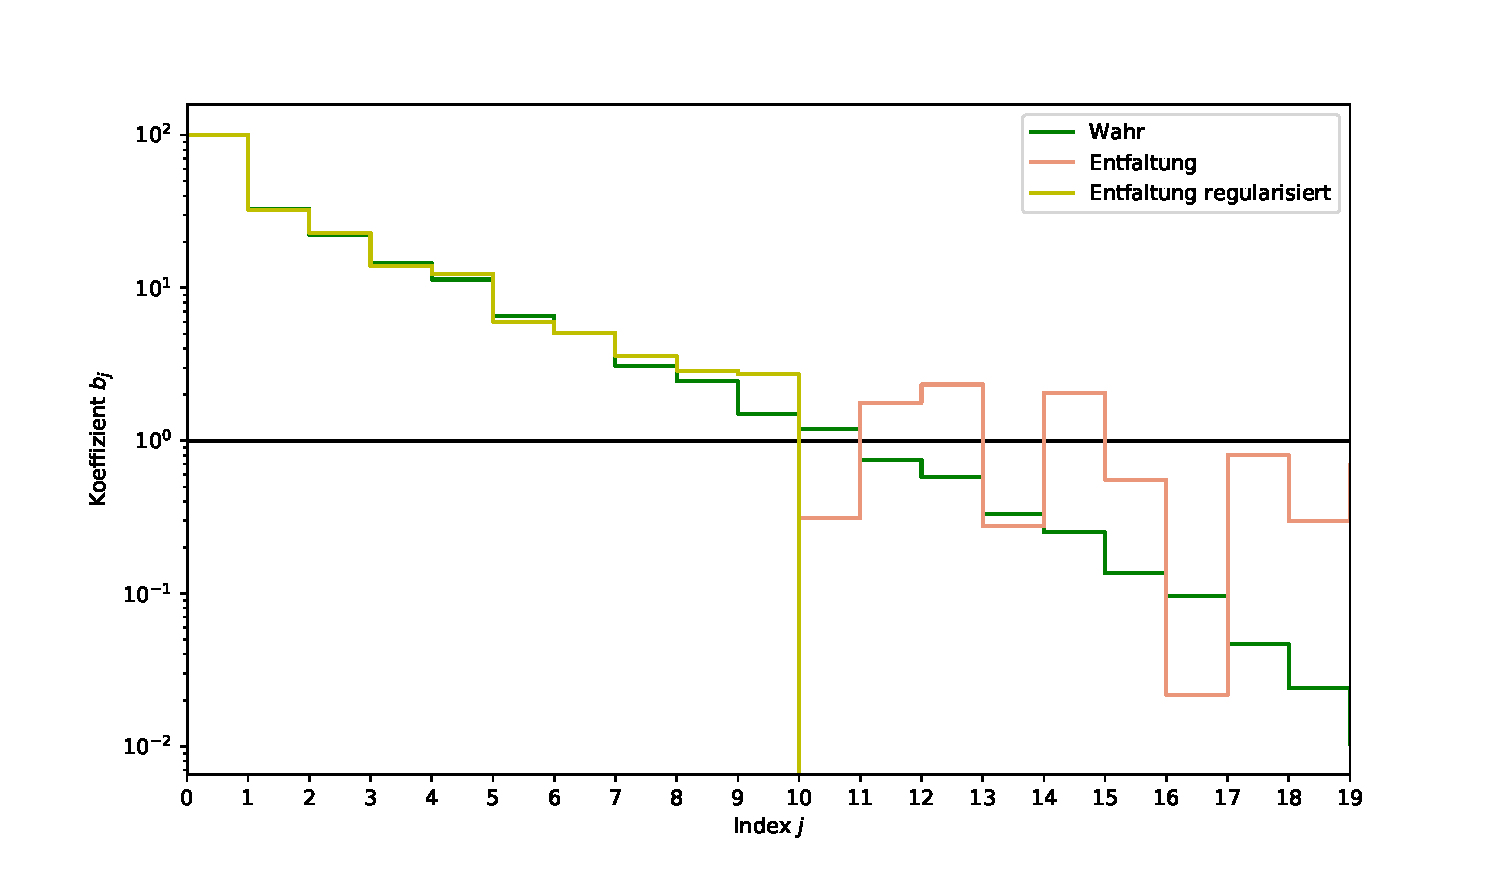
\includegraphics[width=\textwidth]{../A37/Eigenbasis.pdf}
    \caption{Darstellung der Koeffizienten in Eigenbasis.}
    \label{fig:eigenbasis}
\end{figure}
Die schwachen Eigenwerte kleiner als 1 sind, wie in Abbildung~\ref{fig:eigenbasis} zu sehen, sehr instabil. Diese werden zur Regularisierung deswegen auf null gesetzt.
\subsection*{e)}
Die Lösung mit Regularisierung hat, wie in Abbildung~\ref{fig:realbasis} gut erkennbar, deutlich geringere Oszillationen. Außerdem sind ihre Fehler ebenfalls deutlich geringer.
\begin{figure}[H]
    \centering
    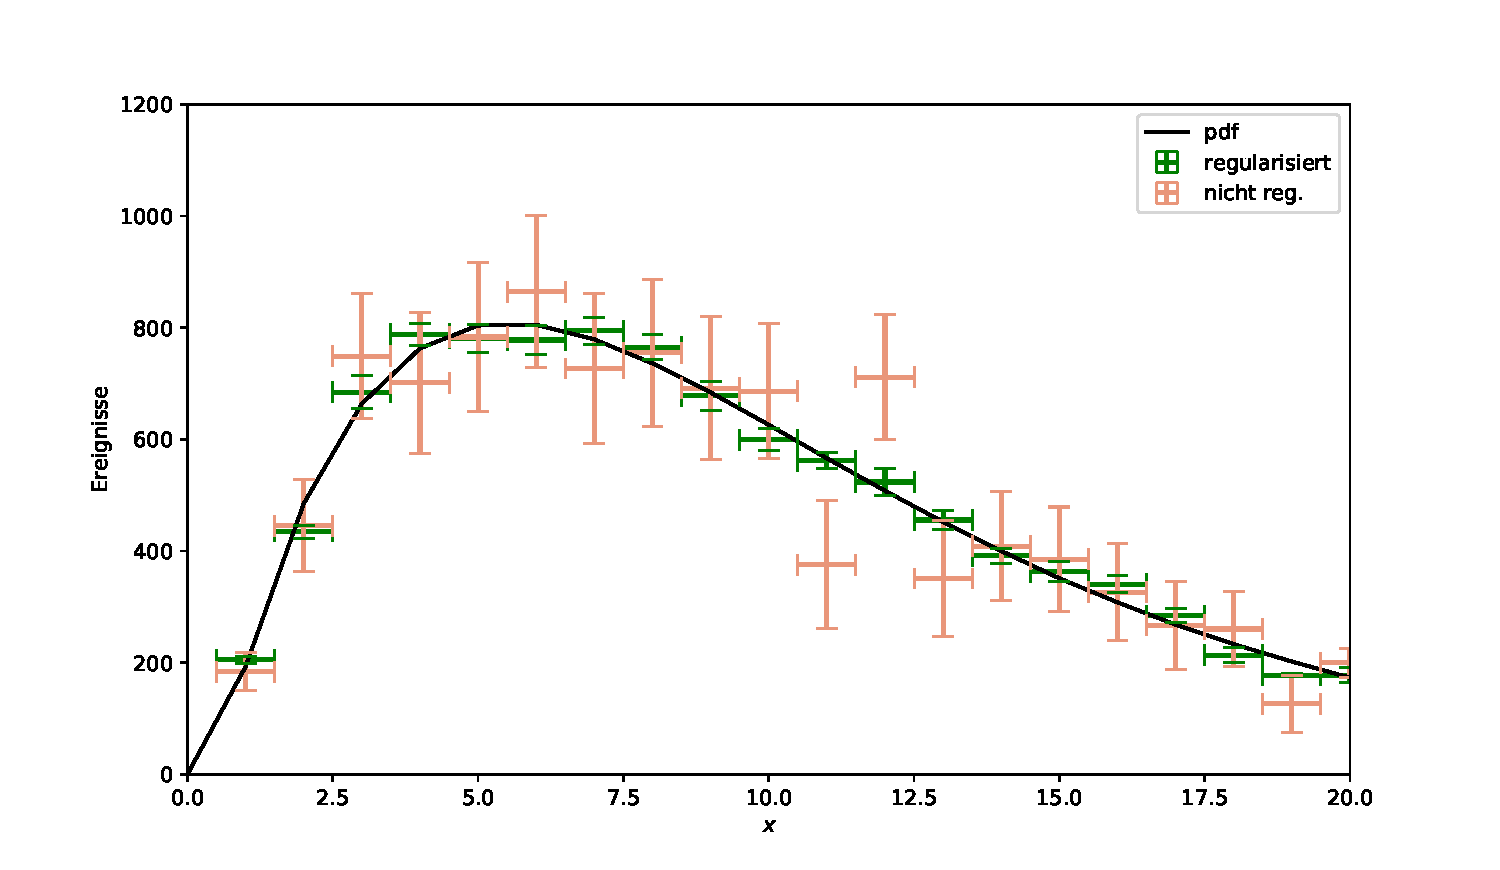
\includegraphics[width=\textwidth]{../A37/Realbasis.pdf}
    \caption{Ergebnis der Entfaltung mit und ohne Regularisierung.}
    \label{fig:realbasis}
\end{figure}
\includepdf[pages=2]{../Rechnungen.pdf}
\FloatBarrier


\section*{Aufgabe 38}
\subsection*{a)}
In den Histogrammen ist eindeutig erkennbar, dass das Attribut \textit{size} die beste Korrelation mit dem Zielattribut \textit{energy\_true} aufweist, daher wird \textit{size} als Attribut zur Entfaltung gewählt.
\begin{figure}[H]
    \centering
    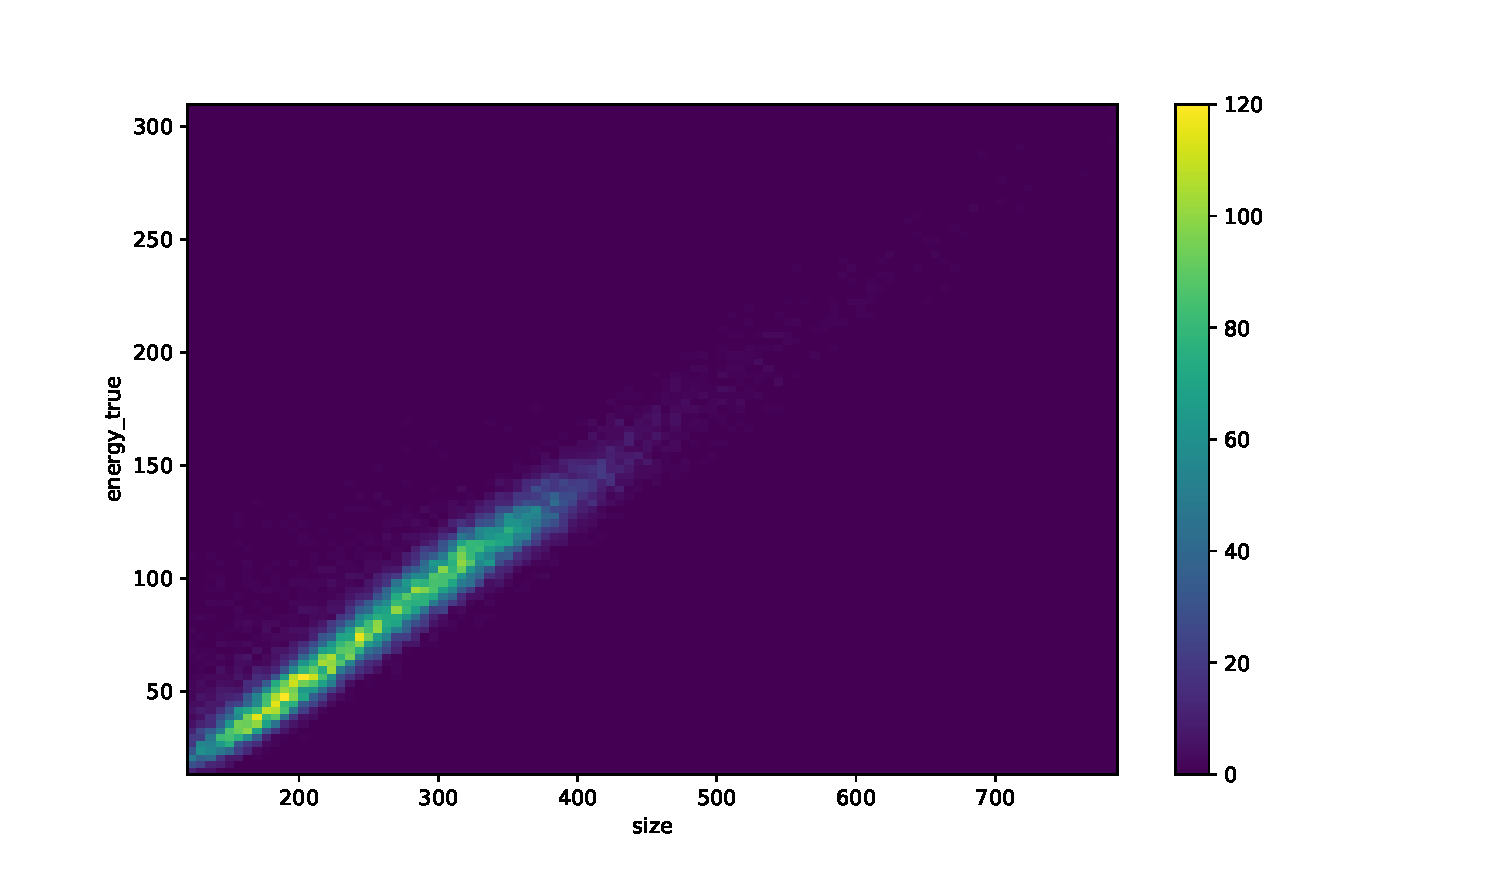
\includegraphics[width=\textwidth]{../A38/A37a_size.pdf}
    \caption{Zwei-dimensionales Histogramm für die Attribute \textit{energy\_true} und \textit{size}.}
    \label{fig:hist_size}
\end{figure}
\begin{figure}[H]
    \centering
    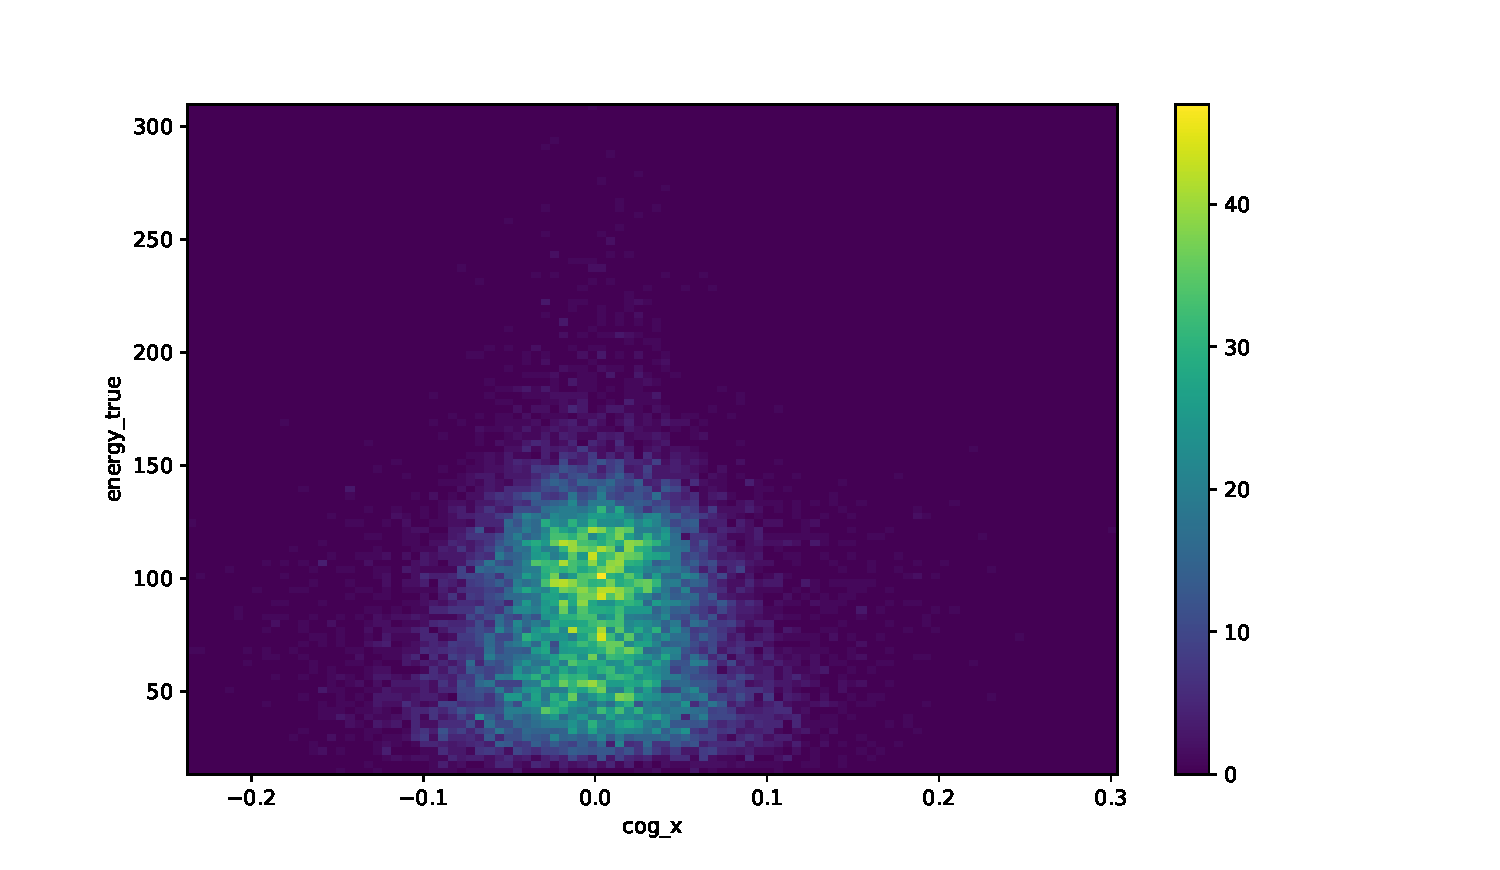
\includegraphics[width=\textwidth]{../A38/A37a_cog_x.pdf}
    \caption{Zwei-dimensionales Histogramm für die Attribute \textit{energy\_true} und \textit{cog\_x}.}
    \label{fig:hist_cog_x)}
\end{figure}
\begin{figure}[H]
    \centering
    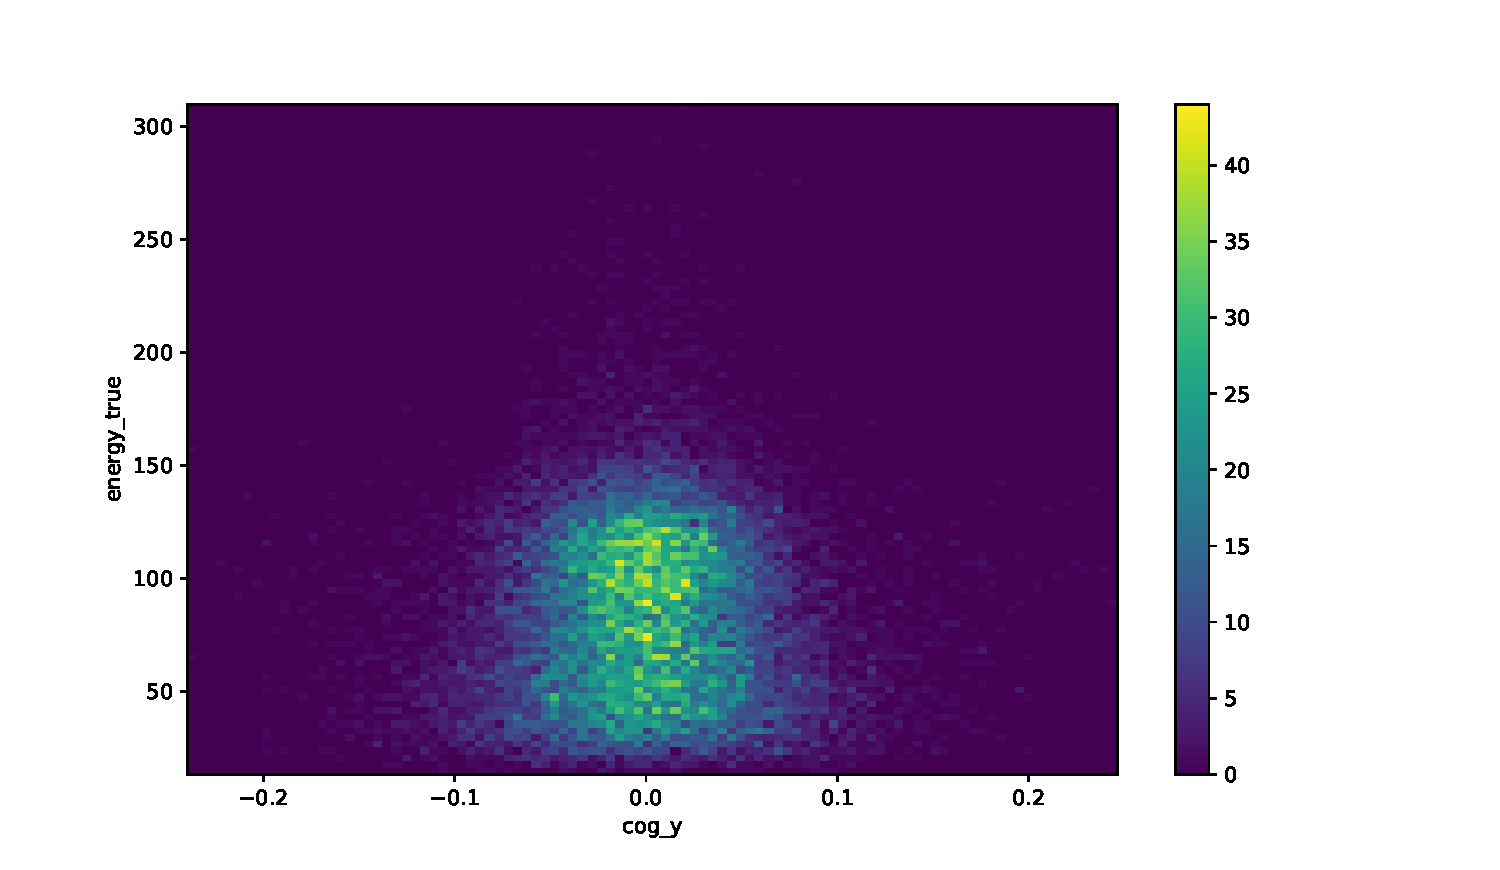
\includegraphics[width=\textwidth]{../A38/A37a_cog_y.pdf}
    \caption{Zwei-dimensionales Histogramm für die Attribute \textit{energy\_true} und \textit{cog\_y}.}
    \label{fig:hist_cog_y}
\end{figure}
\begin{figure}[H]
    \centering
    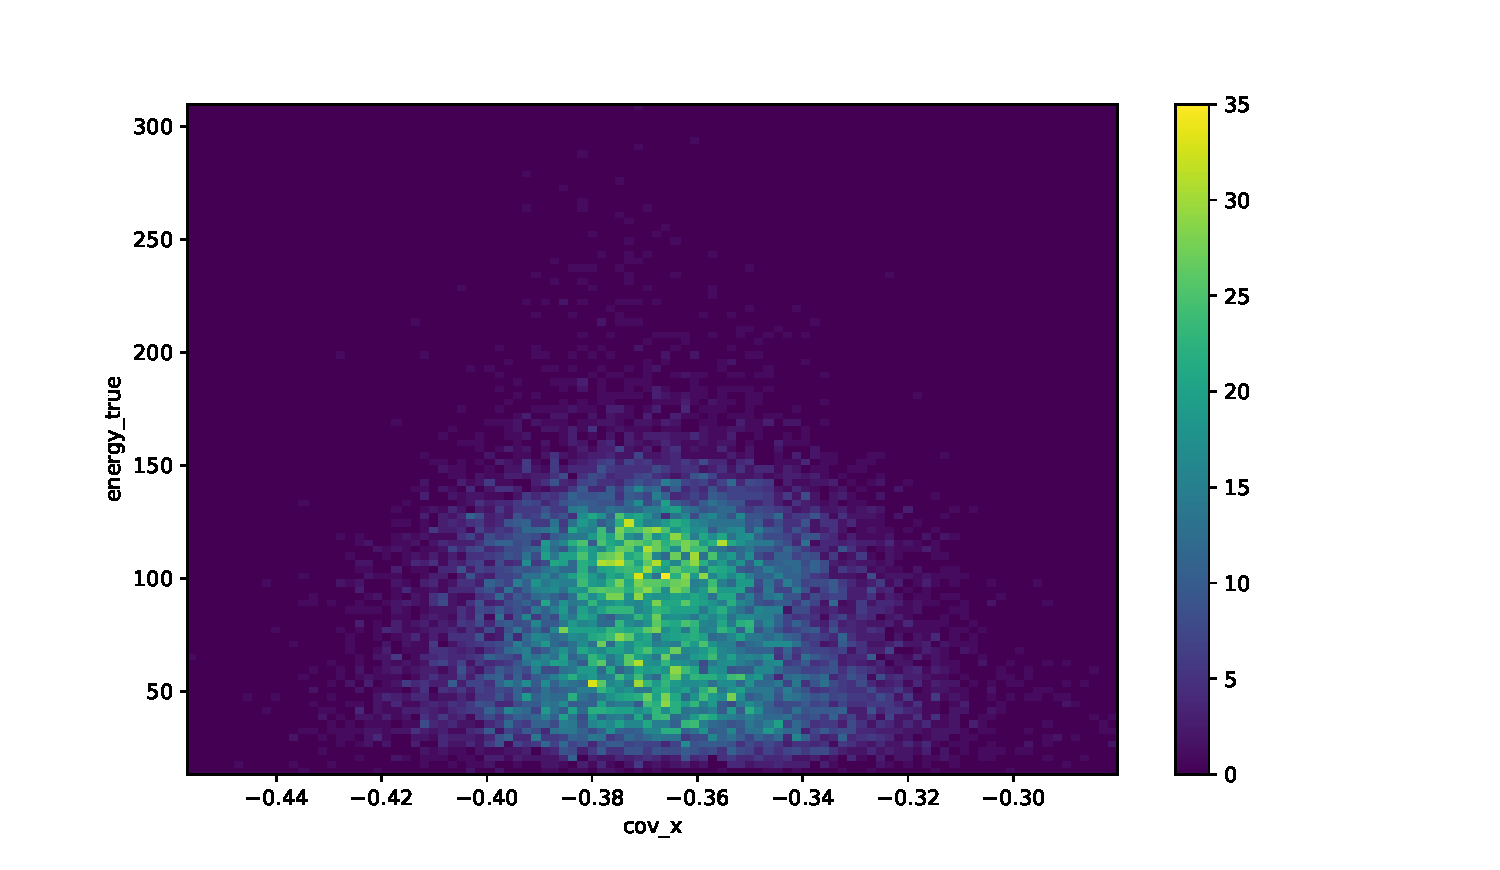
\includegraphics[width=\textwidth]{../A38/A37a_cov_x.pdf}
    \caption{Zwei-dimensionales Histogramm für die Attribute \textit{energy\_true} und \textit{cov\_x}.}
    \label{fig:hist_cov_x}
\end{figure}
\begin{figure}[H]
    \centering
    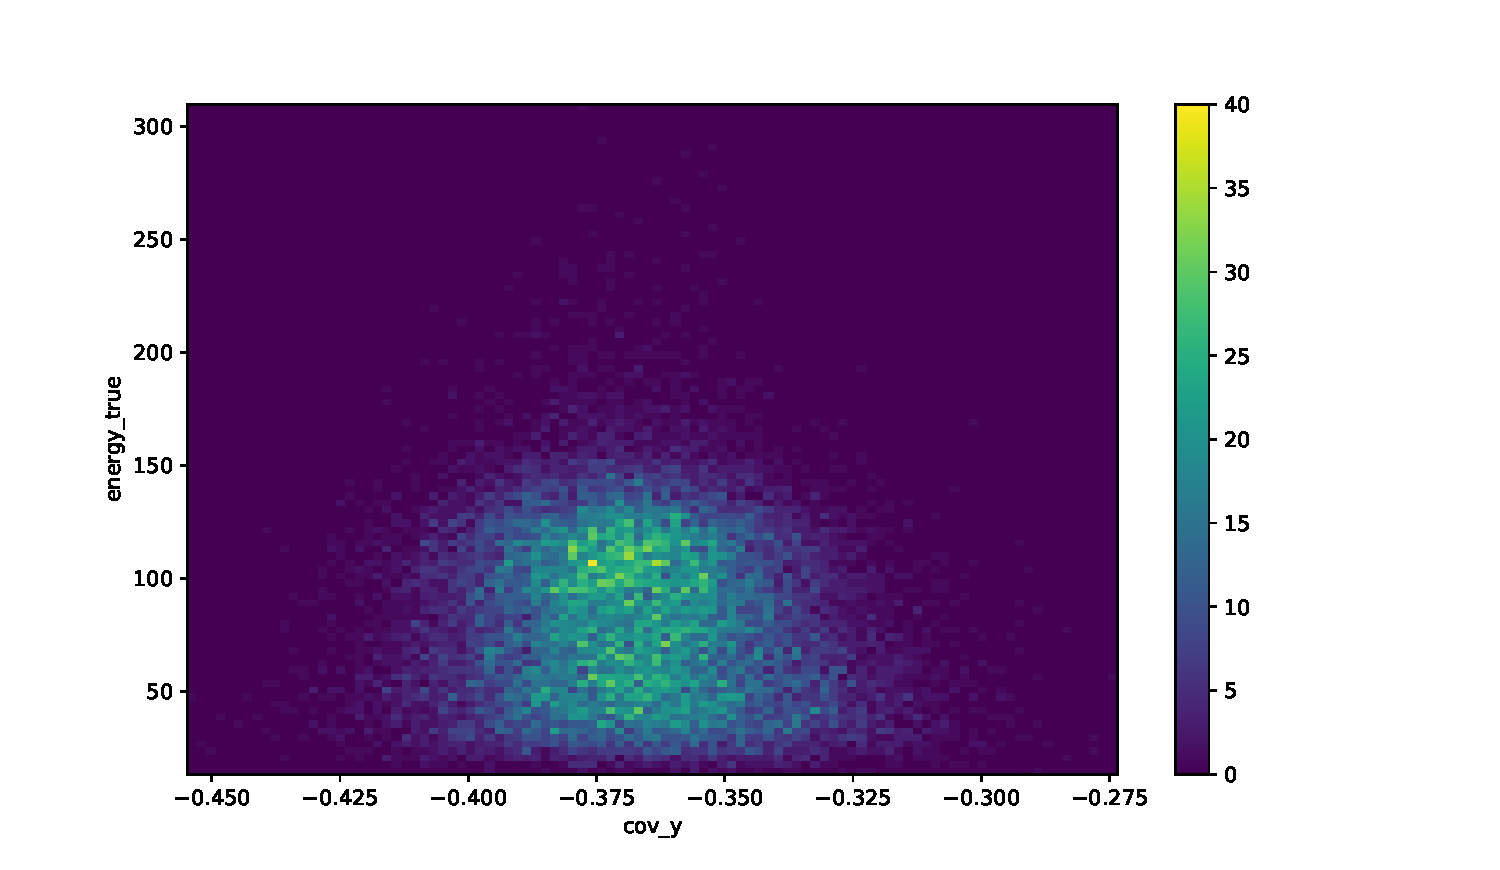
\includegraphics[width=\textwidth]{../A38/A37a_cov_y.pdf}
    \caption{Zwei-dimensionales Histogramm für die Attribute \textit{energy\_true} und \textit{cov\_y}.}
    \label{fig:hist_cov_y}
\end{figure}
\begin{figure}[H]
    \centering
    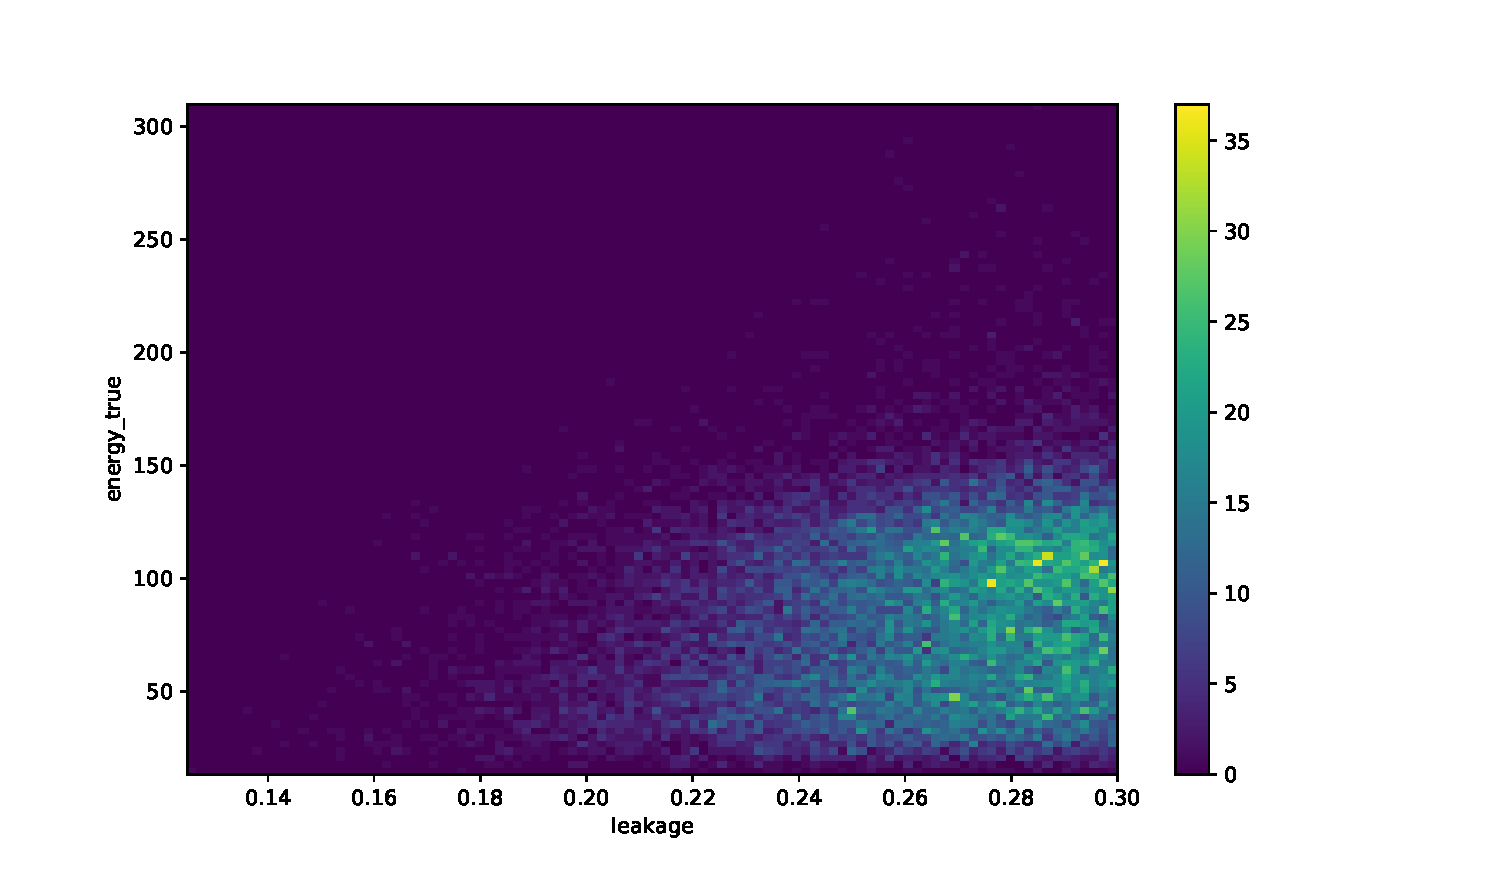
\includegraphics[width=\textwidth]{../A38/A37a_leakage.pdf}
    \caption{Zwei-dimensionales Histogramm für die Attribute \textit{energy\_true} und \textit{leakage}.}
    \label{fig:hist_leackage}
\end{figure}

\subsection*{b)}
Die Migrationsmatrix $A$ ist in Abbildung~\ref{fig:matrix} dargestellt.
\begin{figure}
    \centering
    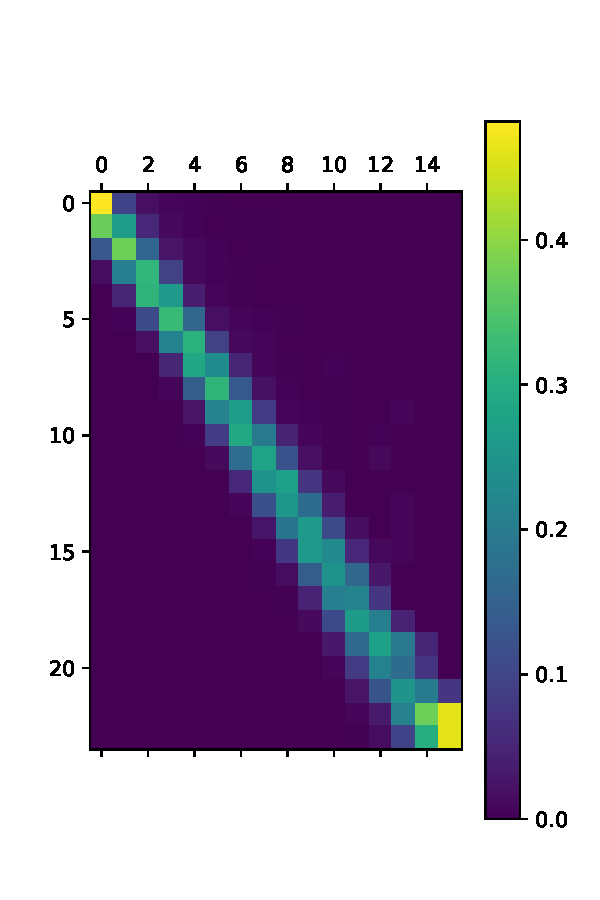
\includegraphics[]{../A38/A37b.pdf}
    \caption{Grafische Darstellung der Migrationsmatrix.}
    \label{fig:matrix}
\end{figure}

\subsection*{e)}
Leider zu wenig Zeit, wir benutzen stattdessen einfach \textit{scipy} zum Minimieren.

\subsection*{f)}
Der Vergleich der verschiedenen Regularisierungsstärken in Abbildung~\ref{fig:38f} zeigt, dass die Regularisierung mit $\tau = 0,001$ am angemessensten erscheint.
\begin{figure}[H]
    \centering
    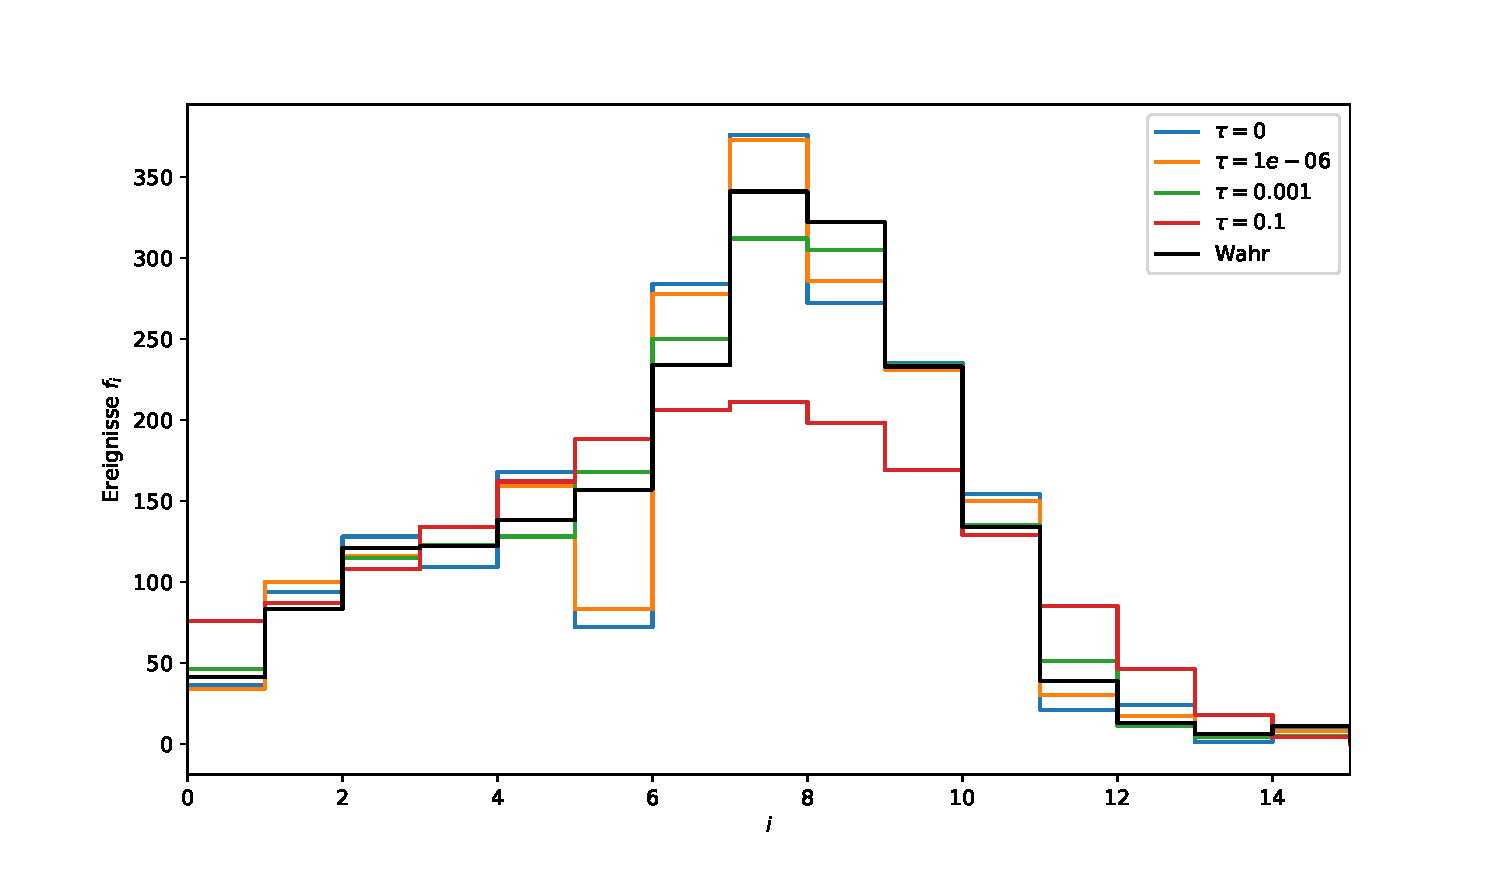
\includegraphics[width=\textwidth]{../A38/A38f.pdf}
    \caption{Ergebnis der Entfaltung mit verschiedenen Regularisierungsstärken $\tau$.}
    \label{fig:38f}
\end{figure}
\includepdf[pages=3]{../Rechnungen.pdf}

\end{document}
